\begin{itemize}
    \item \textbf{Question type distribution}.
        \subitem We sampled 250 questions and manually annotated the set of relevant spans in the passage and the categories of discrete operations that need be performed on the relevant spans to answer the question. \tabref{main_examples} shows the distribution of these categories in the dataset.
    
        \subitem To get a better sense of the question types on the entire dataset, we also curate most frequently occurring 200 bigram and trigram patterns and partition them into different categories based on domain knowledge. For example, the patterns with words ``longest", ``shortest", and ``farthest" etc. would require sorting. This heuristic-based approximate question distribution is shown in \tabref{main_examples}. We also show a drill down on different lingusitic patterns
   
   \item In order to discern the level of complexity needed to understand the passage, we perform a distance based analysis on the spans collected as part of our annotations described above. We found that on an average two spans need to be considered to answer a question and the average distance between these spans is 23 words. \figref{span_highlight} shows that the candidate spans are quite far illustrating the importance of complex passage understanding with coreference resolution.
  
  \item Distribution of answers
%   \begin{table}[t]
%   \centering
%     \begin{tabularx}{\linewidth}{p{1.95cm}p{0.5cm}p{4.25cm}}
%     \toprule
%     {\bf Answer Type} & {\bf Percentage} & {\bf Example}\\
%      \midrule
%      NUMBER & 59.1 & 12 \\
%      PERSON & 13.9 & 12 \\ 
%      OTHER ENTITIES & 9.7 & 12 \\ 
%      DATE & 5.4 & 12 \\ 
%      \bottomrule
%     \end{tabularx}
%   \end{table}
    % \item What's \emph{not} in the data: common sense inference, except for lexical relationships (e.g., grandfather $==$ mother's father).  Some questions require knowledge of scoring in sports; there are enough examples of these that the model at least has a chance of learning this from the data.
\end{itemize}

\begin{figure}
    \centering
    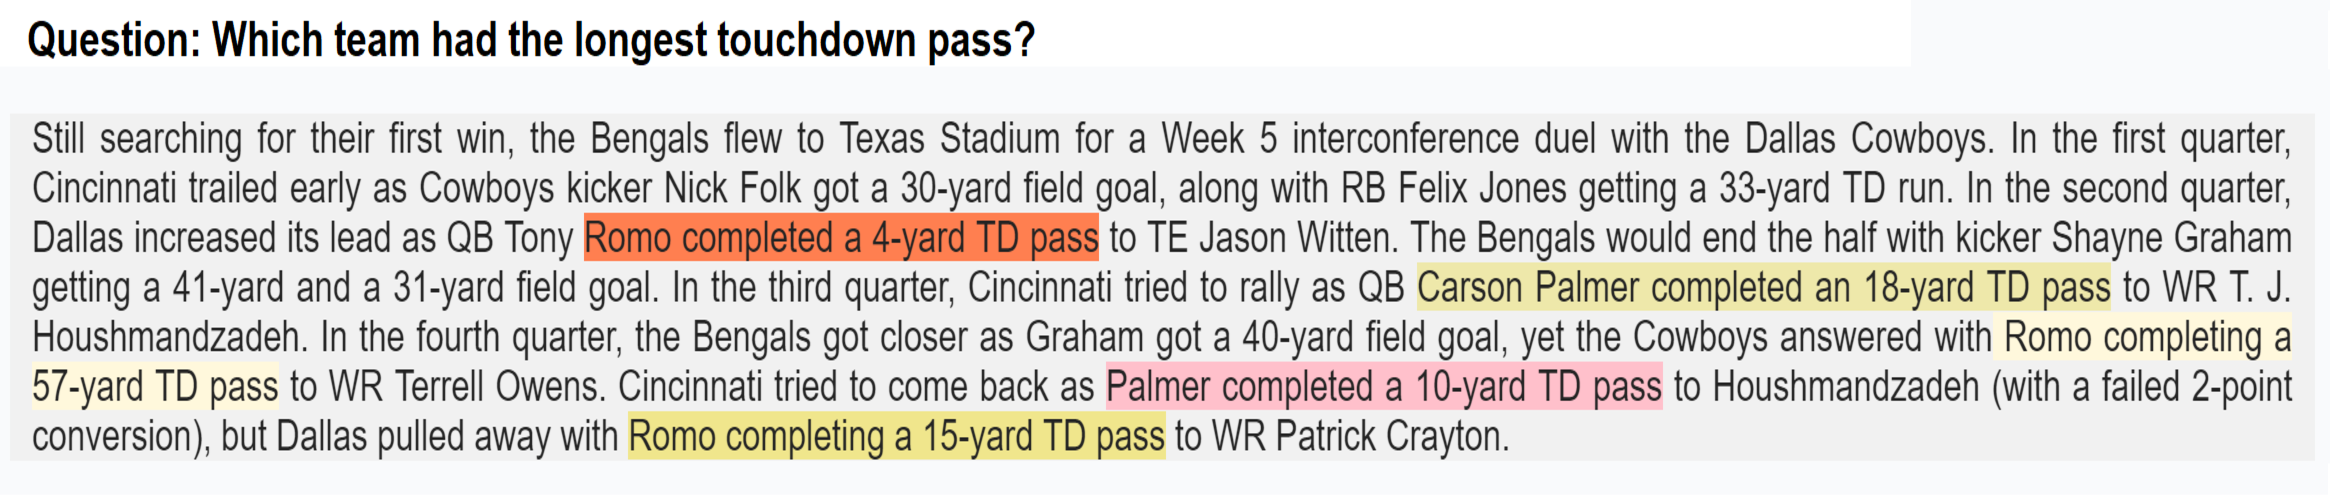
\includegraphics[width=0.5\textwidth]{images/highlights_sort.png}
    \caption{Highlighted candidate spans}
    \label{fig:span_highlight}
\end{figure}
